\documentclass[10pt]{exam}
\usepackage[hon]{template-for-exam}
\usepackage{pgfplots,multicol,cclicenses,hyperref}
\pgfplotsset{
    compat=1.18,
    reg/.append style={
        xmin =-4.5,
        xmax =4.5,
        ymin =-4.5,
        ymax = 4.5,
        axis lines = center,
        xtick = {-4,...,4},
        ytick = {-4,...,4},
        height = 6cm,
        width = 6cm,
        grid = major,
        grid style = {thick, dotted},
        tick label style = {font=\small}
      },
    pulseplot/.append style={
      xmin =-6.5,
      xmax = 6.5,
      ymin =-2.5,
      ymax = 2.5,
      axis lines = center,
      xtick = {-6,...,6},
      ytick = {-2,...,2},
      height = 5cm,
      width = 7.5cm,
      grid = major,
      grid style = {thick, dotted},
      tick label style = {font=\small}
    },
    standingwave/.append style={
      xmin =0,
      xmax = 12,
      ymin =-2.5,
      ymax = 2.5,
      axis y line = box,
      axis x line = center,
      x axis line style=-,
      xtick = {0,...,12},
      ytick = {-2,...,2},
      height = 3cm,
      width = 9cm,
      grid = major,
      grid style = {thick, dotted},
      xticklabels = {},
      yticklabels = {},
    },
    myplot/.append style={
      smooth,domain=-6:6,samples=50,thick
    },
    beatplot/.append style={
      smooth,domain=-0:1.3,samples=100,thick
    }
  }
\pgfmathdeclarefunction{gauss}{2}{%
  \pgfmathparse{1/(#2*sqrt(2*pi))*exp(-((x-#1)^2)/(2*#2^2))}%
}

\title{Wave Phenomena}
\author{Rohrbach}
\date{\today}

\begin{document}
\maketitle

\section*{Basic Properties}

\vs

\section*{Types of Waves}

\vspace{1em}

\begin{center}
  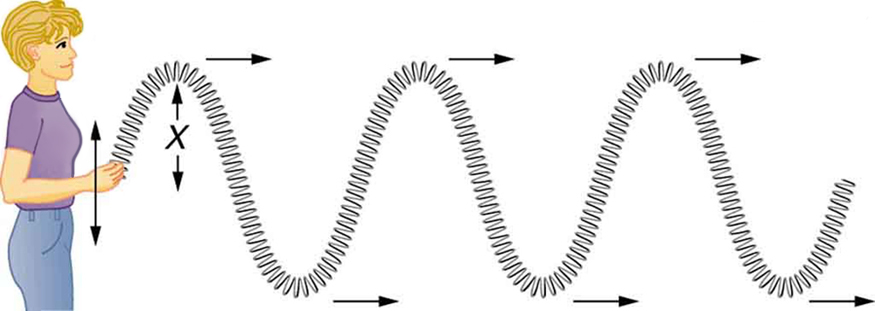
\includegraphics{transverse.jpg}
  
  \vspace{3em}
  
  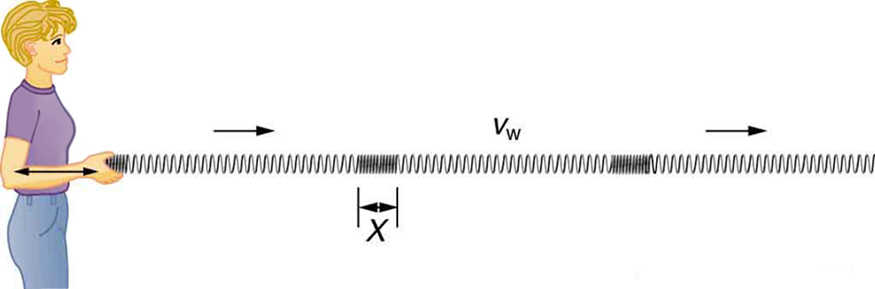
\includegraphics{longitudinal.jpg}

 
\end{center}

{\footnotesize Image Credit: OpenStax \emph{College Physics 2e}. Authored by: P.P Urone, R. Hinrichs, et al. }

{\footnotesize License:} \cc\hspace{-1em}\ccby  {\footnotesize CC BY: Attribution.}

{\footnotesize Retrieved 2024-03-17 from \texttt{\href{https://openstax.org/books/college-physics-2e/pages/16-9-waves}{https://openstax.org/books/college-physics-2e/}} }
\pagebreak

\section*{Superposition}


  \begin{tikzpicture}
    \def\plotsep{4}

    \draw (6.5,3)  -- ++(0,-15);

    \begin{scope}
      \begin{scope}
        \node[anchor=east] at (0,1.8) {$t=\SI{0}{\second}$};
        \begin{axis}[pulseplot]
          \addplot[myplot, ultra thick] {1.3*(gauss(-4,.5)+gauss(4,.5))};
        \end{axis}
      \end{scope}
      
      \begin{scope}[shift={(0,-\plotsep)}]
        \node[anchor=east] at (0,1.8) {$t=\SI{1}{\second}$};
        \begin{axis}[pulseplot]
          \addplot[myplot, ultra thick] {1.3*(gauss(-2,.5)+gauss(2,.5))};
        \end{axis}
      \end{scope}
  
      \begin{scope}[shift={(0,-2*\plotsep)}]
        \node[anchor=east] at (0,1.8) {$t=\SI{2}{\second}$};
        \begin{axis}[pulseplot]
        \end{axis}
      \end{scope}


      \begin{scope}[shift={(0,-3*\plotsep)}]
        \node[anchor=east] at (0,1.8) {$t=\SI{3}{\second}$};
        \begin{axis}[pulseplot]
        \end{axis}
      \end{scope}
  
    \end{scope}

    \begin{scope}[shift={(8,0)}]
      \begin{scope}
        \node[anchor=east] at (0,1.8) {$t=\SI{0}{\second}$};
        \begin{axis}[pulseplot]
          \addplot[myplot, ultra thick] {1.3*(gauss(-4,.5)-gauss(4,.5))};
        \end{axis}
      \end{scope}
      
      \begin{scope}[shift={(0,-\plotsep)}]
        \node[anchor=east] at (0,1.8) {$t=\SI{1}{\second}$};
        \begin{axis}[pulseplot]
          \addplot[myplot, ultra thick] {1.3*(gauss(-2,.5)-gauss(2,.5))};
        \end{axis}
      \end{scope}
  
      \begin{scope}[shift={(0,-2*\plotsep)}]
        \node[anchor=east] at (0,1.8) {$t=\SI{2}{\second}$};
        \begin{axis}[pulseplot]
        \end{axis}
      \end{scope}


      \begin{scope}[shift={(0,-3*\plotsep)}]
        \node[anchor=east] at (0,1.8) {$t=\SI{3}{\second}$};
        \begin{axis}[pulseplot]
        \end{axis}
      \end{scope}
  
    \end{scope}
  \end{tikzpicture}


\section*{Interference}



\begin{center}
  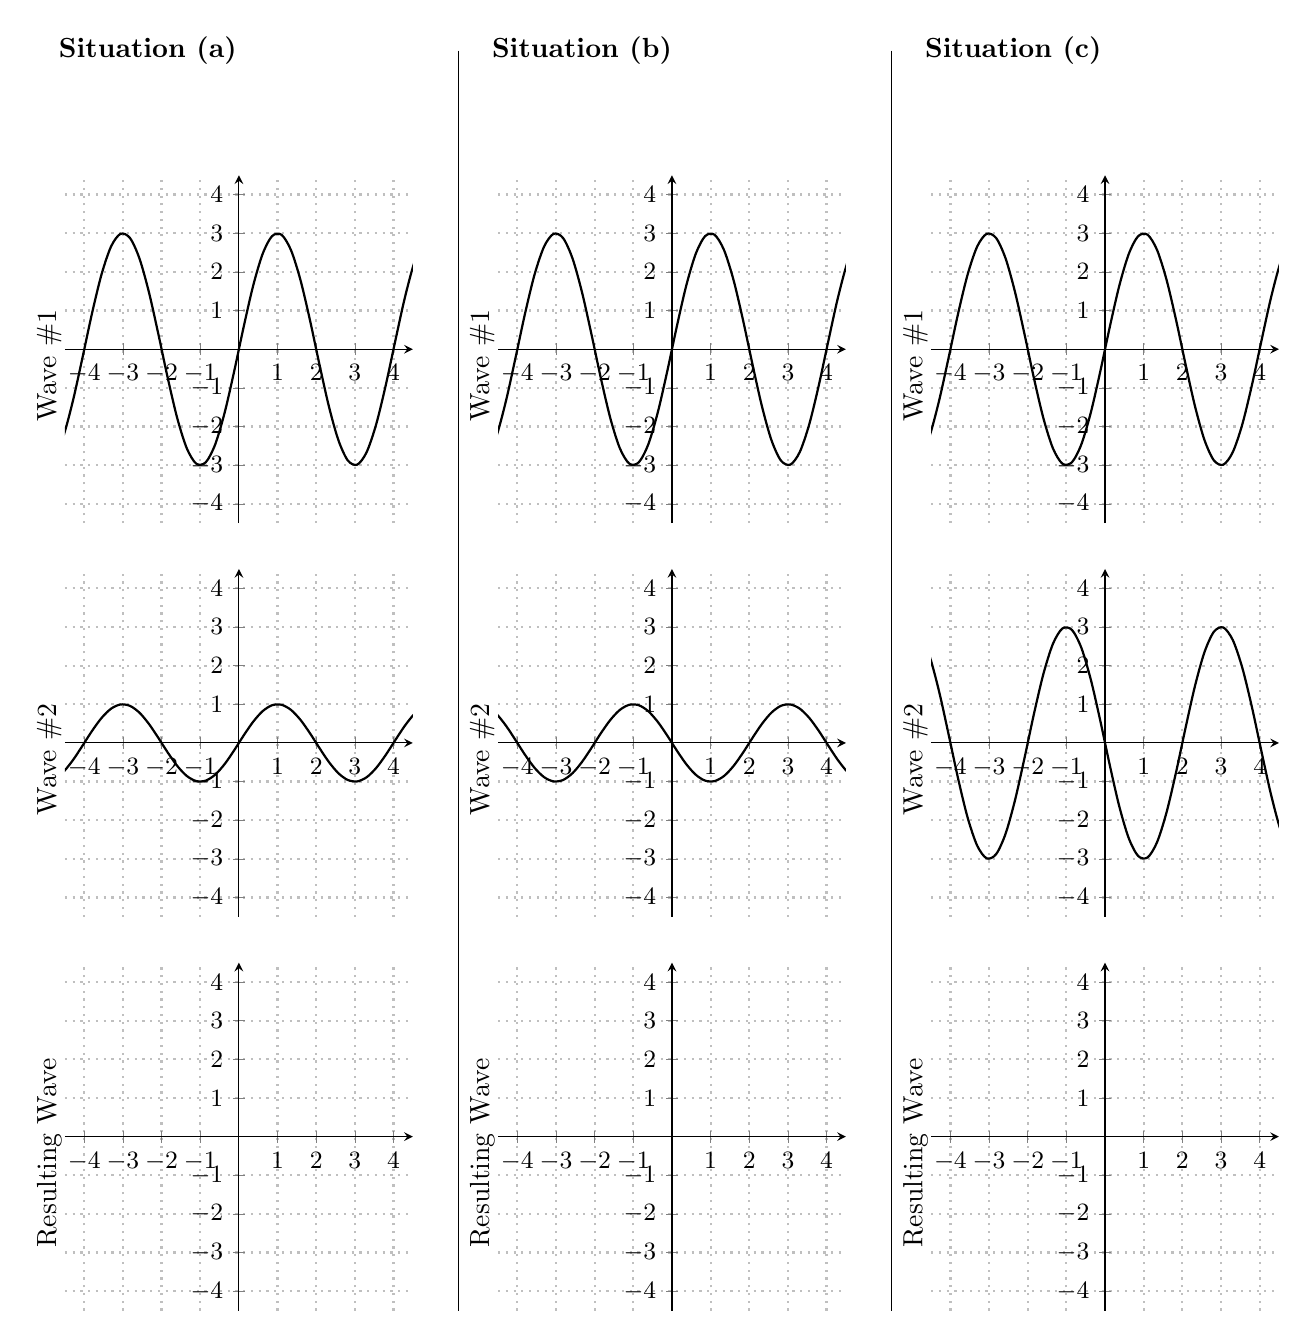
\begin{tikzpicture}
    \draw (5,6)  -- ++(0,-16);
    \draw (10.5,6)  -- ++(0,-16);
  
    \begin{scope}
      \node[anchor=west] at (-.2,6) {\bf Situation (a)};
      \begin{scope}
          \node[rotate=90] at (-.2,2) {Wave \#1};
          \begin{axis}[reg]
            \addplot[myplot] {3*sin(deg(2*pi*x/4))};
          \end{axis}
      \end{scope}
      
      \begin{scope}[shift={(0,-5)}]
        \node[rotate=90] at (-.2,2) {Wave \#2};
        \begin{axis}[reg]
          \addplot[myplot] {1*sin(deg(2*pi*x/4))};
        \end{axis}
      \end{scope}
  
      \begin{scope}[shift={(0,-10)}]
        \node[rotate=90] at (-.2,2) {Resulting Wave};
        \begin{axis}[reg]
        \end{axis}
      \end{scope}
  
    \end{scope}
      
    \begin{scope}[shift={(5.5,0)}]
  
      \node[anchor=west] at (-.2,6) {\bf Situation (b)};
      \begin{scope}
        \node[rotate=90] at (-.2,2) {Wave \#1};
          \begin{axis}[reg]
            \addplot[myplot] {3*sin(deg(2*pi*x/4))};
          \end{axis}
      \end{scope}
      
      \begin{scope}[shift={(0,-5)}]
        \node[rotate=90] at (-.2,2) {Wave \#2};
        \begin{axis}[reg]
          \addplot[myplot] {-1*sin(deg(2*pi*x/4))};
        \end{axis}
      \end{scope}
  
      \begin{scope}[shift={(0,-10)}]
        \node[rotate=90] at (-.2,2) {Resulting Wave};
        \begin{axis}[reg]
        \end{axis}
      \end{scope}
  
    \end{scope}
  
    \begin{scope}[shift={(11,0)}]
  
      \node[anchor=west] at (-.2,6) {\bf Situation (c)};
      \begin{scope}
        \node[rotate=90] at (-.2,2) {Wave \#1};
          \begin{axis}[reg]
            \addplot[myplot] {3*sin(deg(2*pi*x/4))};
          \end{axis}
      \end{scope}
      
      \begin{scope}[shift={(0,-5)}]
        \node[rotate=90] at (-.2,2) {Wave \#2};
        \begin{axis}[reg]
          \addplot[myplot] {-3*sin(deg(2*pi*x/4))};
        \end{axis}
      \end{scope}
  
      \begin{scope}[shift={(0,-10)}]
        \node[rotate=90] at (-.2,2) {Resulting Wave};
        \begin{axis}[reg]
        \end{axis}
      \end{scope}
  
    \end{scope}
  
  \end{tikzpicture}
\end{center}







\pagebreak

\section*{Resonance}

\vs


\begin{tikzpicture}
  \begin{axis}[
    xmin = 0,
    xmax =4.5,
    ymin =0,
    ymax = 4.5,
    axis lines = left,
    xtick = {-10,10},
    ytick = {-10,10},
    height = 5cm,
    width = 6cm,
    grid = none,
    xlabel = {forced frequency},
    ylabel = {amplitude},
  ]
  \end{axis}
\end{tikzpicture}
%
\hfill
%
\begin{tikzpicture}
  \begin{axis}[
    xmin = 0,
    xmax =4.5,
    ymin =0,
    ymax = 4.5,
    axis lines = left,
    xtick = {-10,10},
    ytick = {-10,10},
    height = 5cm,
    width = 6cm,
    grid = none,
    xlabel = {forced frequency},
    ylabel = {amplitude},
  ]
  \end{axis}
\end{tikzpicture} 

\vspace{5em}

\section*{Standing Waves}
``Normal Modes''; ``Harmonics''; ``Overtones''

\vs


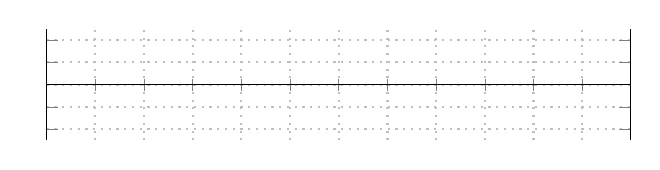
\begin{tikzpicture}
  \begin{axis}[standingwave]
  \end{axis}
\end{tikzpicture}
\vspace{1em}

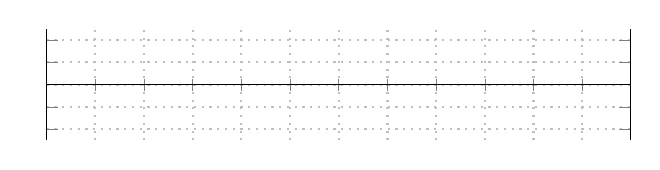
\begin{tikzpicture}
  \begin{axis}[standingwave]
  \end{axis}
\end{tikzpicture}
\vspace{1em}

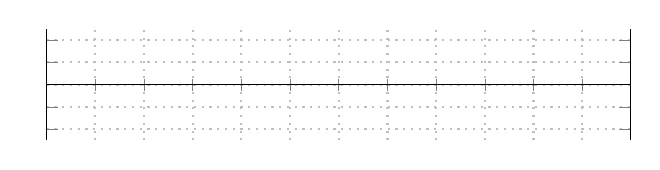
\begin{tikzpicture}
  \begin{axis}[standingwave]
  \end{axis}
\end{tikzpicture}
\vspace{1em}

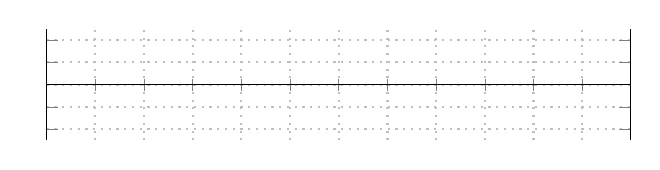
\begin{tikzpicture}
  \begin{axis}[standingwave]
  \end{axis}
\end{tikzpicture}

\vspace{3em}


\pagebreak
\paragraph{Example Problem} The lowest note an open trumpet plays is C (concert B$\flat$) at 466.16 Hz. It turns out that this is actually the second harmonic of the air column in the trumpet

\vspace{1em}

\begin{parts}
  \part Calculate the fundamental frequency of the trumpet.
  \part Calculate the first eight harmonics of the trumpet.
  \part Use the table below to determine which notes these harmonics correspond to.
\end{parts}

\vs


\begin{multicols}{3}
  \footnotesize
  \centering

  \begin{tabular}{ccc}
    Concert & B$\flat$ Trumpet & Frequency \\
    Pitch   &  Pitch & (Hz) \\ 
    \hline\hline
    B$\flat_3$ & C$_4$ & 233.08 \\
    B$_3$ & D$\flat_4$ & 246.94 \\
    C$_4$ & D$_4$ & 261.63 \\
    D$\flat_4$ & E$\flat_4$ & 277.18 \\
    D$_4$ & E$_4$ & 293.66 \\
    E$\flat_4$ & F$_4$ & 311.13 \\
    E$_4$ & G$\flat_4$ & 329.63 \\
    F$_4$ & G$_4$ & 349.23 \\
    G$\flat_4$ & A$\flat_4$ & 369.99 \\
    G$_4$ & A$_4$ & 392.00 \\
    A$\flat_4$ & B$\flat_4$ & 415.30 \\
    A$_4$ & B$_4$ & 440.00 \\
    \hline
  \end{tabular}

  \begin{tabular}{ccc}
    Concert & B$\flat$ Trumpet & Frequency \\
    Pitch   &  Pitch & (Hz) \\ 
    \hline\hline
    B$\flat_4$ & C$_5$ & 466.16 \\
    B$_4$ & D$\flat_5$ & 493.88 \\
    C$_5$ & D$_5$ & 523.25 \\
    D$\flat_5$ & E$\flat_5$ & 554.37 \\
    D$_5$ & E$_5$ & 587.33 \\
    E$\flat_5$ & F$_5$ & 622.25 \\
    E$_5$ & G$\flat_5$ & 659.25 \\
    F$_5$ & G$_5$ & 698.46 \\
    G$\flat_5$ & A$\flat_5$ & 739.99 \\
    G$_5$ & A$_5$ & 783.99 \\
    A$\flat_5$ & B$\flat_5$ & 830.61 \\
    A$_5$ & B$_5$ & 880.00 \\
    \hline
  \end{tabular}

  \begin{tabular}{ccc}
    Concert & B$\flat$ Trumpet & Frequency \\
    Pitch   &  Pitch & (Hz) \\ 
    \hline\hline
    B$\flat_5$ & C$_6$ & 932.33 \\
    B$_5$ & D$\flat_6$ & 987.77 \\
    C$_6$ & D$_6$ & 1046.50 \\
    D$\flat_6$ & E$\flat_6$ & 1108.73 \\
    D$_6$ & E$_6$ & 1174.66 \\
    E$\flat_6$ & F$_6$ & 1244.51 \\
    E$_6$ & G$\flat_6$ & 1318.51 \\
    F$_6$ & G$_6$ & 1396.91 \\
    G$\flat_6$ & A$\flat_6$ & 1479.98 \\
    G$_6$ & A$_6$ & 1567.98 \\
    A$\flat_6$ & B$\flat_6$ & 1661.22 \\
    A$_6$ & B$_6$ & 1760.00 \\
    \hline
    B$\flat_6$ & C$_7$ & 1864.66 \\
    \hline
  \end{tabular}
  
\end{multicols}



\pagebreak 
\section*{Beats}
  
\vspace{10em}
  
\begin{tikzpicture}
  \node at (0,0) 
    {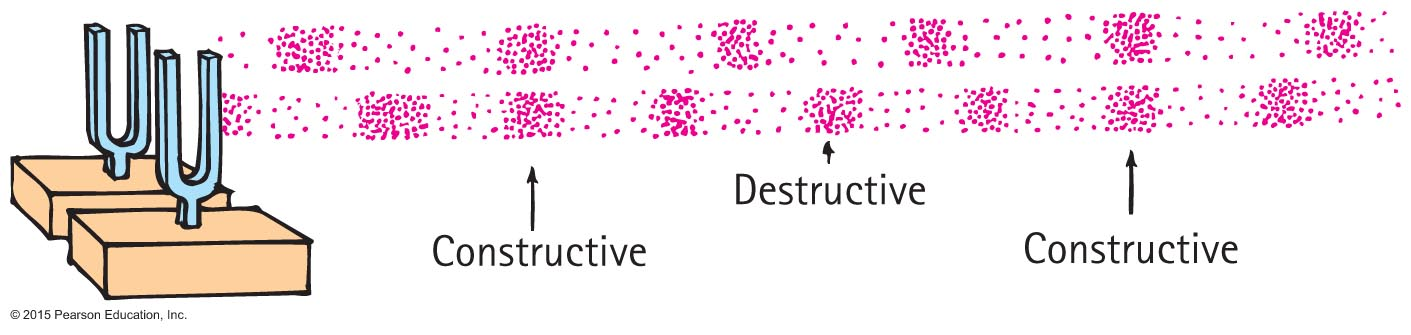
\includegraphics[width=12cm]{Fig20_21.jpg}};
  \fill[white] (-3,-1) rectangle (6,.26);
\end{tikzpicture}

\vspace{3em}

\noindent
Take a look at the illustration below that refers to a wave of frequency 10 Hz being played at the same time as a wave of frequency 12 Hz.

\vspace{1em}

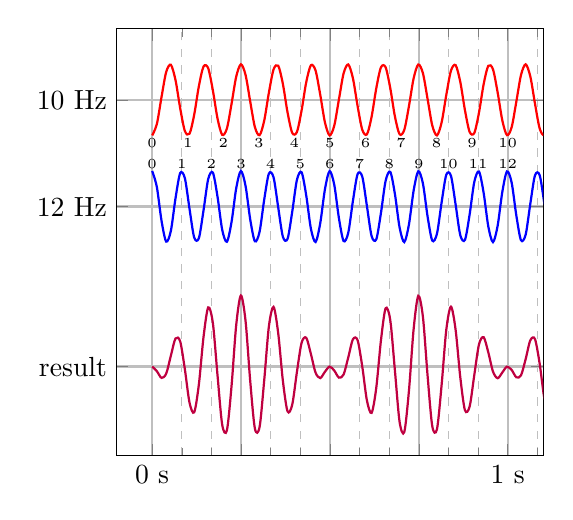
\begin{tikzpicture}
  \begin{axis}[
    xmin=-0.1,
    xmax=1.1,
    ymin=-7,
    ymax=5,
    axis y line = box,
    axis x line = box,
    x axis line style=-,
    xtick = {0,0.25,0.5,0.75,1,1.25},
    ytick = {3,0,-4.5},
    height = 7cm,
    width = 7cm,
    grid = both,
    minor tick num = 2,
    major grid style = {thick},
    minor grid style = {thin, dashed},
    xticklabels = {0 s,,,,1 s,},
    yticklabels = {10 Hz, 12 Hz, result},
  ]
    \addplot[beatplot,red] {-cos(deg(20*pi*x))+3};
    \addplot[beatplot,blue] {cos(deg(24*pi*x))};
    \addplot[beatplot,purple] {-cos(deg(20*pi*x))+cos(deg(24*pi*x))-4.5};
    \pgfplotsinvokeforeach{0,...,10} {
      \node at (0.1*#1,1.8)
        {\tiny #1};
    }
    \pgfplotsinvokeforeach{0,...,12} {
      \node at (#1/12,1.2)
        {\tiny #1};
    }
   
  \end{axis}
  
\end{tikzpicture}
  

\vspace{3em}

\noindent
Draw your own beats!  Draw two bugs jumping on the water.  One bug jumps forward 3 cm each hop; the other bug jumps forward 4 cm each hop.

\begin{tikzpicture}
  \draw[dotted] (0,0) grid[step=0.5] (15,-1.5);
\end{tikzpicture}



\end{document}